\documentclass[12pt,a4paper,oneside]{report}

\usepackage{fontspec}
\setmainfont{Times New Roman}
\renewcommand{\chaptername}{CHƯƠNG}
\renewcommand{\contentsname}{MỤC LỤC}
\renewcommand{\listfigurename}{DANH MỤC HÌNH}
\renewcommand{\listtablename}{DANH MỤC BẢNG}
\renewcommand{\bibname}{TÀI LIỆU THAM KHẢO}
\usepackage{geometry}
\geometry{left=3cm,right=2cm,top=2.5cm,bottom=2.5cm,headheight=15pt}
\usepackage{setspace}
\onehalfspacing
\usepackage{graphicx}
\usepackage{float}
\usepackage{booktabs,tabularx,array,longtable,multirow}
\usepackage{amsmath,amssymb}
\usepackage{tikz}
\usetikzlibrary{arrows.meta,positioning,shapes.geometric,shapes.multipart,fit,calc,backgrounds}
\usepackage{caption}
\usepackage{chngcntr}
\counterwithin{figure}{chapter}
\counterwithin{table}{chapter}
\captionsetup[figure]{name=Hình,position=bottom,justification=centering,font=small,labelfont=bf}
\captionsetup[table]{name=Bảng,position=top,justification=centering,font=small,labelfont=bf}
\usepackage{enumitem}
\setlist{nosep,leftmargin=1.2cm}
\usepackage{url}
\usepackage[hidelinks]{hyperref}
\usepackage{fancyhdr}
\usepackage{titlesec}
\usepackage{microtype}
\usepackage{listings}
\usepackage{xcolor}
\definecolor{travelgreen}{HTML}{14685E}
\definecolor{travelgold}{HTML}{F4A11A}
\definecolor{softgreen}{HTML}{EAF5EF}
\definecolor{softgold}{HTML}{FFF5DE}
\definecolor{ink}{HTML}{253C3A}
\pagestyle{fancy}
\fancyhf{}
\fancyhead[L]{\small Báo cáo Trí tuệ nhân tạo -- Travel Path}
\fancyhead[R]{\small \leftmark}
\fancyfoot[C]{\thepage}
\renewcommand{\headrulewidth}{0.4pt}
\titleformat{\chapter}[display]{\bfseries\centering\color{travelgreen}}{\Large CHƯƠNG \thechapter}{0.4em}{\LARGE}
\titleformat{\section}{\large\bfseries\color{travelgreen}}{\thesection}{0.7em}{}
\titleformat{\subsection}{\normalsize\bfseries\color{ink}}{\thesubsection}{0.7em}{}
\setlength{\parindent}{1.25cm}
\setlength{\parskip}{0.15em}
\renewcommand{\arraystretch}{1.2}
\newcolumntype{Y}{>{\raggedright\arraybackslash}X}
\newcommand{\VND}{\,\text{đ}}
\newcommand{\code}[1]{\texttt{#1}}

\begin{document}

% -----------------------------------------------------------------------------
% BÌA
% -----------------------------------------------------------------------------
\begin{titlepage}
\begin{tikzpicture}[remember picture,overlay]
  \draw[line width=1.0pt] ([xshift=1.15cm,yshift=-1.1cm]current page.north west) rectangle ([xshift=-1.15cm,yshift=1.1cm]current page.south east);
  \draw[line width=0.45pt,color=travelgreen] ([xshift=1.25cm,yshift=-1.2cm]current page.north west) rectangle ([xshift=-1.25cm,yshift=1.2cm]current page.south east);
\end{tikzpicture}
\centering
\vspace*{1cm}
{\bfseries BỘ GIÁO DỤC VÀ ĐÀO TẠO\par}
\vspace{0.2cm}
{\bfseries TRƯỜNG ĐẠI HỌC KIẾN TRÚC ĐÀ NẴNG\par}
\vspace{0.2cm}
{\bfseries KHOA: CÔNG NGHỆ THÔNG TIN\par}
\vspace{0.35cm}
\rule{2.8cm}{0.5pt}\,o0o\,\rule{2.8cm}{0.5pt}

\vspace{0.8cm}

\includegraphics[width=2.2cm]{Bao_cao_Travel_Path_assets/logo_truong.png}

\vspace{0.7cm}
{\Large\bfseries BÁO CÁO TRÍ TUỆ NHÂN TẠO\par}
\vspace{0.7cm}
{\large\bfseries Đề tài: XÂY DỰNG HỆ THỐNG TRỢ LÝ DU LỊCH\par}
\vspace{0.15cm}
{\large\bfseries THÔNG MINH VỚI AI\par}

\vspace{0.8cm}
\begin{tabular}{>{\bfseries}r @{}c l}
Giảng viên hướng dẫn & : & TS. Đỗ Phúc Hào \\
\addlinespace[0.25cm]
Sinh viên thực hiện & : & Bùi Thị Quỳnh Như \\
 & & Cao Trúc Ny \\
\addlinespace[0.2cm]
Mã số sinh viên & : & 2351220202 \\
 & & 2251220201 \\
\addlinespace[0.2cm]
Lớp & : & 23CT4 \\
\end{tabular}

\vfill
{\bfseries ĐÀ NẴNG -- 2026\par}
\vspace*{0.8cm}
\end{titlepage}

\pagenumbering{roman}
\chapter*{LỜI CAM ĐOAN}
Nhóm thực hiện cam đoan báo cáo này được xây dựng phục vụ học phần Trí tuệ nhân tạo, nội dung mô tả dựa trên mã nguồn và tài liệu tham khảo được liệt kê ở cuối báo cáo. Các hình chụp giao diện được dùng để minh họa sản phẩm trong quá trình phát triển; các sơ đồ thiết kế được vẽ lại bằng TikZ trong LaTeX. Những số liệu tính toán trong ví dụ được ghi rõ là ví dụ minh họa, không được xem là phép đo hiệu năng hay kết quả kiểm thử thực nghiệm.

\chapter*{LỜI CẢM ƠN}
Nhóm xin chân thành cảm ơn TS. Đỗ Phúc Hào đã hướng dẫn về cách trình bày báo cáo, yêu cầu giải thích ý nghĩa của từng bảng, hình và kết quả, cũng như góp ý về cấu trúc ba chương. Nhóm cũng cảm ơn các nguồn tài liệu kỹ thuật và dữ liệu du lịch công khai đã hỗ trợ quá trình tìm hiểu, thiết kế và xây dựng Travel Path.

\chapter*{TÓM TẮT}
Travel Path là ứng dụng web hỗ trợ người dùng tạo lịch trình du lịch theo điểm đến, số ngày, số người, ngân sách và sở thích. Hệ thống kết hợp giao diện trò chuyện, bộ lập lịch dựa trên dữ liệu địa điểm, thành phần gợi ý, ước tính chi phí và các chức năng tài khoản. Phần diễn giải ngôn ngữ tự nhiên có thể sử dụng mô hình Ollama chạy cục bộ; khi mô hình không sẵn sàng, chương trình có nhánh xử lý theo luật. Lịch trình hiển thị theo ngày và khung giờ; các địa điểm ưu tiên dữ liệu có địa chỉ, giá và trạng thái đủ điều kiện sử dụng.

Báo cáo trình bày tổng quan bài toán, phương pháp và cấu trúc hệ thống, sau đó phân tích các giao diện và phép tính chi phí. Tài liệu có ba chương theo yêu cầu: (1) Giới thiệu tổng quan về bài toán; (2) Phương pháp và hệ thống thực hiện; (3) Kết quả. Sơ đồ được tạo bằng TikZ; bảng được dàn bằng môi trường LaTeX; mỗi hình và bảng đều có số theo chương và phần diễn giải. Các ví dụ chi phí minh họa quy tắc tính của mã nguồn, không khẳng định kết quả chạy kiểm thử.

\vspace{0.5cm}
\noindent\textbf{Từ khóa:} trợ lý du lịch, lập lịch trình, gợi ý địa điểm, ngân sách, FastAPI, PostgreSQL, Ollama.

\tableofcontents
\listoffigures
\listoftables
\clearpage
\pagenumbering{arabic}

% =============================================================================
\chapter{GIỚI THIỆU TỔNG QUAN VỀ BÀI TOÁN}
% =============================================================================

\section{Bối cảnh}
Du lịch là hoạt động cần phối hợp nhiều quyết định nhỏ: chọn điểm đến, xác định thời gian, tìm chỗ lưu trú, chọn điểm tham quan và sắp xếp bữa ăn. Khách du lịch thường phải tham khảo nhiều trang và tự kiểm tra khoảng cách, giá, giờ mở cửa. Khi thay đổi số ngày hoặc ngân sách, người dùng phải rà soát lại lịch trình. Đây là bài toán tổ chức thông tin và ra quyết định có nhiều ràng buộc, phù hợp với một ứng dụng có thể tiếp nhận yêu cầu bằng ngôn ngữ tự nhiên và chuyển chúng thành dữ liệu có cấu trúc.

Theo Cục Thống kê, Việt Nam đón khoảng 21,2 triệu lượt khách quốc tế trong năm 2025, tăng 20,4\% so với năm trước [3]. Chính phủ đã đặt mục tiêu phát triển du lịch theo hướng chuyên nghiệp, chất lượng và gắn với ứng dụng công nghệ trong Chiến lược phát triển du lịch Việt Nam đến năm 2030 [1]. Những dữ kiện này cho thấy quy mô hoạt động du lịch và định hướng chuyển đổi số đều đáng được quan tâm. Cục Du lịch Quốc gia Việt Nam cũng duy trì một bảng thống kê khách quốc tế riêng [4]. Khi chuẩn hóa dữ liệu địa điểm, cần lưu ý các thay đổi đơn vị hành chính được quy định tại Nghị quyết 202/2025/QH15 [5]. Từ đó, nhóm chọn nghiên cứu một trợ lý lập kế hoạch nhằm gom các bước tra cứu và sắp lịch vào một quy trình. Đây là lý do chọn đề tài ở góc độ kỹ thuật; các số liệu vĩ mô không được diễn giải thành bằng chứng trực tiếp rằng mọi du khách đều cần sản phẩm này.

\begin{table}[H]
\centering
\caption{Dữ kiện bối cảnh dùng để xác lập lý do chọn đề tài}
\label{tab:context}
\begin{tabularx}{\textwidth}{p{3.3cm}p{3.2cm}Y}
\toprule
\textbf{Dữ kiện} & \textbf{Giá trị/định hướng} & \textbf{Ý nghĩa đối với đề tài} \\
\midrule
Khách quốc tế đến Việt Nam năm 2025 & Khoảng 21,2 triệu lượt; tăng 20,4\% [3] & Cho thấy hoạt động du lịch có quy mô lớn; đặt ra nhu cầu tổ chức thông tin chuyến đi, nhưng không tự nó chứng minh nhu cầu thị trường của ứng dụng cụ thể. \\
Chiến lược phát triển du lịch đến 2030 & Phát triển chuyên nghiệp, chất lượng, bền vững và ứng dụng công nghệ [1] & Cung cấp căn cứ định hướng để khảo sát cách công nghệ hỗ trợ chuẩn bị hành trình. \\
Luật Du lịch 2017 & Quy định khung hoạt động du lịch và quyền, nghĩa vụ liên quan [2] & Là nguồn nền tảng khi mô tả phạm vi thông tin du lịch và yêu cầu cung cấp thông tin có trách nhiệm. \\
\bottomrule
\end{tabularx}
\end{table}
\noindent Bảng~\ref{tab:context} tách số liệu thống kê khỏi định hướng chính sách để tránh suy diễn quá mức. Số lượt khách cho biết quy mô dòng khách; chiến lược và luật cho biết bối cảnh quản lý. Hai loại căn cứ này hỗ trợ lập luận chọn đề tài nhưng không thay thế khảo sát người dùng hay đánh giá hiệu quả sản phẩm.

\section{Lý do chọn đề tài}
Nhóm lựa chọn đề tài vì ba lý do. Thứ nhất, yêu cầu du lịch được diễn đạt tự do nhưng cần chuyển thành tham số rõ ràng như điểm đến, số ngày, số người, ngân sách và sở thích. Thứ hai, lịch trình cần đồng thời thỏa mãn nhiều tiêu chí: địa điểm phù hợp, giờ hoạt động, thời gian nghỉ, bữa ăn, quãng đường và mức chi. Thứ ba, hệ thống tạo cơ hội vận dụng kiến thức trí tuệ nhân tạo, hệ gợi ý, xử lý ngôn ngữ, cơ sở dữ liệu không gian, thiết kế web và bảo mật tài khoản vào một sản phẩm tích hợp.

Việc chọn đề tài cũng có giới hạn: dữ liệu địa điểm và giá trên mạng có thể thiếu, cũ hoặc không đồng nhất; lịch trình tự động chỉ là gợi ý. Do đó, ứng dụng cần thể hiện nguồn/giá theo dữ liệu sẵn có, báo phần chưa đủ dữ liệu, và để người dùng tiếp tục điều chỉnh thay vì trình bày ước tính như báo giá cam kết.

\section{Phát biểu bài toán}
Đầu vào là yêu cầu chuyến đi của một người dùng, có thể được gửi dưới dạng câu chat hoặc các trường biểu mẫu. Hệ thống cần nhận biết thông tin quan trọng, tìm dữ liệu địa điểm tương ứng, sắp xếp hoạt động thành lịch trình theo ngày và tính chi phí dự kiến. Nếu người dùng bổ sung sở thích hoặc yêu cầu đổi nơi lưu trú, hệ thống cần cập nhật plan theo yêu cầu mới. Kết quả cần dễ đọc, có thể lưu vào lịch sử tài khoản và tải xuống dưới dạng PDF.

Có thể mô hình hóa đầu vào của bài toán như sau:
\[
  q=(d,n,p,b,S),
\]
trong đó $d$ là điểm đến, $n$ là số ngày, $p$ là số người, $b$ là ngân sách toàn chuyến và $S$ là tập sở thích. Hệ thống tìm lịch trình $I$ và ước tính chi phí $C(I)$; mục tiêu là tạo một lịch trình phù hợp với $q$, giảm di chuyển không cần thiết và hạn chế vượt ngân sách khi dữ liệu cho phép. Vì dữ liệu giá có thể thiếu, hệ thống không thể luôn bảo đảm $C(I)\leq b$; giao diện cần nói rõ trường hợp vượt ngân sách hoặc chưa đủ dữ liệu.

\section{Mục tiêu}
\begin{itemize}
  \item Xây dựng giao diện web cho phép người dùng trao đổi bằng tiếng Việt và nhập thông tin chuyến đi.
  \item Tạo lịch trình theo ngày, phân loại hoạt động và đề xuất địa điểm từ dữ liệu có sẵn.
  \item Tính chi phí lưu trú, ăn uống và tổng chuyến đi theo quy tắc thống nhất.
  \item Hỗ trợ đăng ký bằng OTP email, đăng nhập, khôi phục mật khẩu, lưu lịch sử plan và chức năng quản trị.
  \item Tổ chức hệ thống theo các thành phần có thể chạy cục bộ bằng Docker Compose và có cấu hình để xem xét triển khai web sau này.
\end{itemize}

\section{Phạm vi và giả định}
\begin{table}[H]
\centering
\caption{Phạm vi thực hiện và các giới hạn của đề tài}
\label{tab:scope}
\begin{tabularx}{\textwidth}{p{3cm}Y Y}
\toprule
\textbf{Hạng mục} & \textbf{Trong phạm vi} & \textbf{Giới hạn/giả định} \\
\midrule
Giao diện & Trang trò chuyện, lập kế hoạch, địa điểm, khách sạn, lịch sử, tài khoản và quản trị. & Ảnh chụp trong báo cáo phản ánh bản giao diện thử nghiệm trong quá trình phát triển, không khẳng định mọi nội dung ảnh là dữ liệu cập nhật tại ngày nộp. \\
Lập lịch & Xếp địa điểm thành khung giờ và ngày; gợi ý theo sở thích, địa bàn, giá và giờ hoạt động. & Chất lượng bị giới hạn bởi độ đầy đủ và độ chính xác của DB; kết quả là gợi ý để người dùng rà soát. \\
Chi phí & Ước lượng lưu trú, ăn uống và tổng chuyến đi. & Giá đầu vào có thể là một mức, khoảng giá hoặc không có; không thay thế xác nhận trực tiếp từ cơ sở dịch vụ. \\
AI hội thoại & Dùng mô hình Ollama cục bộ khi sẵn sàng, có nhánh luật dự phòng. & Không xem mô hình ngôn ngữ là nguồn dữ liệu thực tế; dữ liệu địa điểm được lấy từ hệ thống dữ liệu. \\
Triển khai & Cấu hình chạy cục bộ bằng Docker Compose. & Chưa gắn tên miền hay máy chủ công khai; triển khai sản xuất chưa được xác nhận trong báo cáo này. \\
\bottomrule
\end{tabularx}
\end{table}
\noindent Bảng~\ref{tab:scope} phân biệt phần đã có trong cấu trúc dự án với giới hạn của bản đồ án. Cách phân định này ngăn việc hiểu nhầm rằng đề tài đã triển khai dịch vụ thương mại công khai hoặc bảo đảm dữ liệu giá luôn mới. Phần AI xử lý ngôn ngữ và phần dữ liệu địa điểm là hai nguồn trách nhiệm khác nhau: mô hình giúp diễn giải yêu cầu, còn địa điểm/giá phải truy xuất từ dữ liệu hệ thống.

\section{Phương pháp thực hiện}
Nhóm khảo sát yêu cầu và cấu trúc dự án; phân tích mô-đun frontend, API, cơ sở dữ liệu và thành phần AI; mô tả luồng xử lý; sau đó đối chiếu các giao diện đã có với yêu cầu nghiệp vụ. Thiết kế hệ gợi ý được trình bày ở mức tổng hợp các tiêu chí mà mã nguồn sử dụng, không gán điểm chất lượng nếu không có phép đo. Ví dụ số học được tính trực tiếp từ công thức mô tả. Tại thời điểm lập báo cáo, các bảng kiểm tra ở Chương~3 được gọi là kịch bản nghiệm thu đề xuất; báo cáo không tuyên bố chúng đã được chạy tự động.

\section{Các nghiên cứu và nền tảng liên quan}
Hệ gợi ý thường kết hợp thông tin người dùng, thuộc tính đối tượng và đánh giá tương đồng. Resnick và Varian trình bày vai trò của recommender system trong việc chọn lọc thông tin [6]. Burke phân loại các phương pháp gợi ý lai và phân tích cách kết hợp nguồn tín hiệu [7]. Trong Travel Path, các tiêu chí thực dụng gồm sở thích, địa bàn, khoảng cách, giá và giờ hoạt động; đây là bộ lọc/ranking theo dữ liệu hiện có chứ không phải mô hình học sâu được huấn luyện trên lịch sử đánh giá lớn.

FastAPI cung cấp cơ chế xây dựng API và tài liệu OpenAPI [8,9,10]; PostgreSQL lưu trữ dữ liệu quan hệ, còn PostGIS mở rộng khả năng truy vấn không gian [11,12]. Docker Compose mô tả các dịch vụ phối hợp trong môi trường cục bộ [13]. Ollama cung cấp API hội thoại cho mô hình cục bộ [14]. Các nền tảng này hỗ trợ triển khai kiến trúc; bản thân chúng không chứng minh độ chính xác của gợi ý. Về bảo mật, báo cáo đối chiếu nguyên tắc lưu mật khẩu bằng hàm băm chuyên dụng, xác thực phiên và quản lý thông tin xác thực với OWASP và tài liệu Python [15--18].

\section{Bố cục báo cáo}
Báo cáo gồm đúng ba chương. Chương~1 giới thiệu bối cảnh, lý do chọn đề tài, mục tiêu, phạm vi và nền tảng liên quan. Chương~2 mô tả yêu cầu, kiến trúc, dữ liệu, thuật toán và cách triển khai. Chương~3 trình bày giao diện, kết quả chức năng theo mã nguồn, ví dụ phân tích chi phí, kịch bản nghiệm thu, hạn chế và kết luận.

% =============================================================================
\chapter{PHƯƠNG PHÁP VÀ HỆ THỐNG THỰC HIỆN}
% =============================================================================

\section{Công nghệ sử dụng}
Frontend được xây dựng bằng HTML, CSS và JavaScript; backend dùng Python và FastAPI. Dữ liệu chính dùng PostgreSQL/PostGIS; dự án có adapter tùy chọn cho MongoDB. Docker Compose điều phối frontend Nginx, backend, PostgreSQL/PostGIS, Ollama và tiến trình thu thập giá. Các thành phần này được dùng vì chúng tách giao diện, nghiệp vụ, lưu trữ và mô hình ngôn ngữ thành các phần có thể cấu hình riêng. FastAPI cung cấp giao diện API có thể mô tả bằng OpenAPI [8--10]; PostGIS hỗ trợ kiểu dữ liệu và truy vấn địa lý [12].

\begin{table}[H]
\centering
\caption{Vai trò các công nghệ chính trong Travel Path}
\label{tab:tech}
\small
\begin{tabularx}{\textwidth}{p{3.2cm}p{3.2cm}Y}
\toprule
\textbf{Công nghệ} & \textbf{Thành phần} & \textbf{Vai trò trong đồ án} \\
\midrule
HTML/CSS/JS & Frontend & Hiển thị chat, kế hoạch, bản đồ thông tin địa điểm, tài khoản và lịch sử. \\
Python + FastAPI & Backend & Cung cấp API xác thực, lập kế hoạch, địa điểm, lịch sử người dùng và quản trị. \\
\shortstack[l]{PostgreSQL /\\ PostGIS} & Cơ sở dữ liệu & Lưu tài khoản, địa điểm và thông tin vị trí; hỗ trợ truy vấn không gian. \\
Ollama & Thành phần AI cục bộ & Diễn giải câu chat; có đường xử lý dự phòng nếu mô hình không sẵn sàng. \\
Docker Compose/Nginx & Môi trường chạy & Điều phối dịch vụ và chuyển tiếp yêu cầu giao diện đến API trong môi trường cục bộ. \\
OSRM & Dịch vụ định tuyến tùy chọn & Tính tuyến đường khi dịch vụ có thể truy cập; hệ thống có thể dùng ước lượng khoảng cách dự phòng. \\
\bottomrule
\end{tabularx}
\normalsize
\end{table}
\noindent Bảng~\ref{tab:tech} cho thấy các công nghệ được chọn theo vai trò chứ không thay thế lẫn nhau. API giữ nghiệp vụ và quyền truy cập tập trung ở backend; cơ sở dữ liệu lưu trạng thái bền vững; frontend chỉ trình bày và gửi yêu cầu. Việc dùng OSRM là tùy chọn, vì vậy khoảng cách dự phòng cần được hiểu là xấp xỉ chứ không phải tuyến đường thực.

\section{Yêu cầu hệ thống}
\subsection{Tác nhân}
\begin{itemize}
  \item \textbf{Khách chưa đăng nhập:} xem trang tài khoản, đăng ký và xác thực OTP.
  \item \textbf{Người dùng:} đăng nhập, tạo/chỉnh sửa/xóa/tải plan, xem lịch sử plan và cập nhật sở thích.
  \item \textbf{Quản trị viên:} xem danh sách tài khoản và một số thông tin thống kê đăng nhập theo vai trò được cấp.
\end{itemize}

\subsection{Yêu cầu chức năng}
\begin{table}[H]
\centering
\caption{Yêu cầu chức năng và ánh xạ đến thành phần hệ thống}
\label{tab:req}
\begin{tabularx}{\textwidth}{p{1.5cm}p{5.1cm}Y}
\toprule
\textbf{Mã} & \textbf{Yêu cầu} & \textbf{Thành phần liên quan} \\
\midrule
F01 & Đăng ký bằng email, tên đăng nhập, mật khẩu nhập lại và OTP. & Frontend tài khoản; API OTP; bảng xác minh đang chờ. \\
F02 & Đăng nhập bằng email và mật khẩu; chặn trang chính khi chưa xác thực. & API đăng nhập/phiên; middleware frontend. \\
F03 & Quên mật khẩu bằng OTP và thiết lập lại mật khẩu. & API gửi, xác minh OTP và cập nhật mật khẩu. \\
F04 & Tiếp nhận yêu cầu chuyến đi từ chat hoặc biểu mẫu. & Giao diện chat/planner; bộ diễn giải yêu cầu. \\
F05 & Tạo lịch trình theo điểm đến, ngày, người, ngân sách, sở thích. & API lập kế hoạch; bộ gợi ý và lập lịch. \\
F06 & Tính và trình bày chi phí; nêu trường hợp vượt ngân sách hoặc thiếu giá. & Hàm ước tính; giao diện tổng hợp chi phí. \\
F07 & Lưu lịch sử plan theo tài khoản; tải bản kế hoạch PDF; xóa plan bằng câu chat. & API lịch sử; frontend xuất PDF và xử lý ý định chat. \\
F08 & Quản trị viên xem thông tin tài khoản và thống kê liên quan. & API và trang quản trị có kiểm soát vai trò. \\
\bottomrule
\end{tabularx}
\end{table}
\noindent Bảng~\ref{tab:req} nhóm chức năng theo hành trình sử dụng. Việc ánh xạ giúp truy nguyên yêu cầu về nơi triển khai trong ứng dụng và phát hiện được chức năng cần xem xét riêng, chẳng hạn PDF là thao tác đầu ra ở giao diện còn quyền đọc lịch sử phải do backend xác minh.

\subsection{Yêu cầu phi chức năng}
Hệ thống cần cung cấp phản hồi dễ hiểu khi thiếu dữ liệu, không hiển thị mật khẩu trong giao diện kết quả, bảo vệ trang theo phiên đăng nhập và vai trò, hạn chế thử OTP quá dồn dập, đồng thời giữ được lịch sử của người dùng. Các yêu cầu này liên quan trực tiếp tới bảo mật xác thực và phiên làm việc; OWASP khuyến nghị dùng cơ chế lưu mật khẩu phù hợp và quản lý phiên an toàn [15--17]. Giao diện phải bố trí được nội dung trên màn hình nhỏ, nhưng báo cáo này không tuyên bố đã đo khả năng tiếp cận hay hiệu năng trên mọi thiết bị.

\section{Kiến trúc tổng thể}
\begin{figure}[H]
\centering
\resizebox{0.94\textwidth}{!}{\begin{tikzpicture}[node distance=0.9cm and 1.0cm,box/.style={draw=travelgreen,rounded corners=4pt,fill=softgreen,align=center,minimum width=3.5cm,minimum height=1.05cm},store/.style={draw=travelgreen,ellipse,fill=softgold,align=center,minimum width=3.5cm,minimum height=1cm},arrow/.style={-{Latex[length=2.5mm]},thick,draw=travelgreen}]
\node[box] (user) {Người dùng / Quản trị viên\\Trình duyệt web};
\node[box,below=of user] (front) {Frontend\\HTML · CSS · JavaScript · Nginx};
\node[box,below=of front] (api) {Backend API\\FastAPI · xác thực · nghiệp vụ};
\node[box,left=of api] (ai) {Diễn giải yêu cầu\\Ollama hoặc luật dự phòng};
\node[box,right=of api] (plan) {Lập lịch và ước tính\\Gợi ý · khoảng cách · chi phí};
\node[store,below=of api] (db) {PostgreSQL / PostGIS\\tài khoản · địa điểm · lịch sử};
\node[box,below=of plan] (route) {OSRM tùy chọn\\tuyến đường / ước lượng};
\draw[arrow] (user)--(front); \draw[arrow] (front)--node[right,font=\small]{HTTP API} (api);
\draw[arrow] (api)--(ai); \draw[arrow] (ai)--(api);
\draw[arrow] (api)--(plan); \draw[arrow] (plan)--(api);
\draw[arrow] (api)--(db); \draw[arrow] (db)--(api);
\draw[arrow] (plan)--(route); \draw[arrow] (route)--(plan);
\end{tikzpicture}}
\caption{Kiến trúc các thành phần của Travel Path}
\label{fig:architecture}
\end{figure}
Hình~\ref{fig:architecture} thể hiện luồng giữa trình duyệt, backend và các dịch vụ hỗ trợ. Backend là nơi điều phối vì xác thực, truy vấn dữ liệu và tính chi phí cần dùng chung quy tắc. Ollama chỉ hỗ trợ diễn giải câu chat; dữ liệu địa điểm vẫn được lấy từ cơ sở dữ liệu. Khi OSRM không khả dụng, hệ thống có phương án ước lượng, vì thế khoảng cách hiển thị khi đó có độ tin cậy thấp hơn tuyến đường theo mạng lưới đường.

\section{Thiết kế dữ liệu}
Các bảng dữ liệu địa điểm và vùng hành chính hỗ trợ lọc theo địa bàn; dữ liệu địa điểm có thể mang tọa độ, giá, nguồn ảnh và trạng thái xử lý. Các bản ghi thu thập được chia trạng thái để chỉ những bản ghi đủ thông tin mới được đưa vào luồng gợi ý. Nhóm bảng tài khoản được khởi tạo ở backend gồm người dùng, phiên làm việc, OTP xác minh email, OTP đặt lại mật khẩu và các plan đã lưu.

\begin{figure}[H]
\centering
\resizebox{0.94\textwidth}{!}{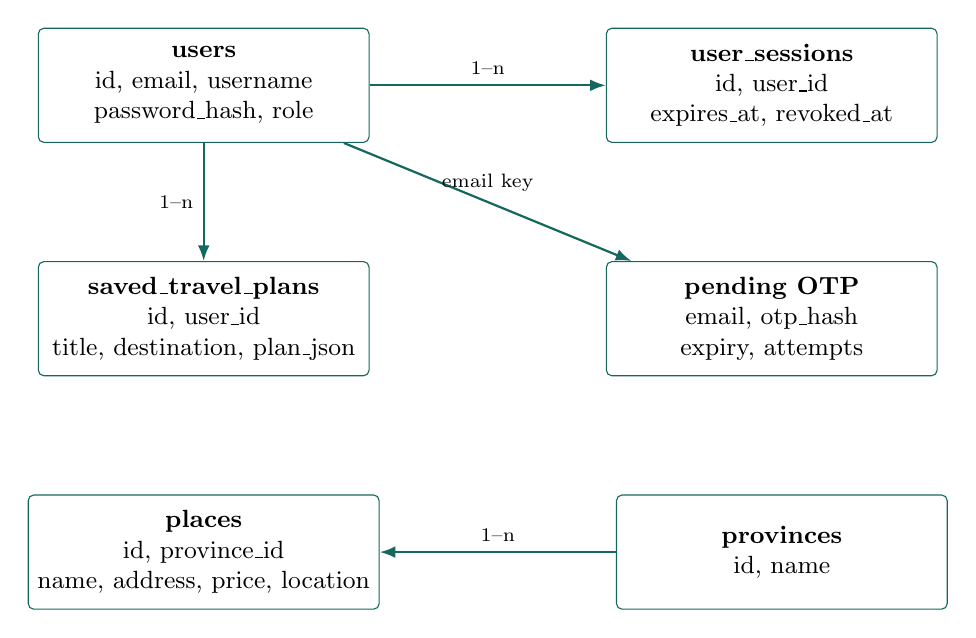
\begin{tikzpicture}[node distance=1.5cm and 3.0cm,entity/.style={draw=travelgreen,rounded corners=2pt,fill=white,minimum width=4.2cm,minimum height=1.45cm,align=center,font=\small},rel/.style={-{Latex[length=2mm]},thick,draw=travelgreen}]
\node[entity] (users) {\textbf{users}\\id, email, username\\password\_hash, role};
\node[entity,right=of users] (sessions) {\textbf{user\_sessions}\\id, user\_id\\expires\_at, revoked\_at};
\node[entity,below=of users] (plans) {\textbf{saved\_travel\_plans}\\id, user\_id\\title, destination, plan\_json};
\node[entity,right=of plans] (otp) {\textbf{pending OTP}\\email, otp\_hash\\expiry, attempts};
\node[entity,below=of plans] (places) {\textbf{places}\\id, province\_id\\name, address, price, location};
\node[entity,right=of places] (provinces) {\textbf{provinces}\\id, name};
\draw[rel] (users)--node[above,font=\scriptsize]{1--n}(sessions);
\draw[rel] (users)--node[left,font=\scriptsize]{1--n}(plans);
\draw[rel] (provinces)--node[above,font=\scriptsize]{1--n}(places);
\draw[rel] (users)--node[above,font=\scriptsize]{email key}(otp);
\end{tikzpicture}}
\caption{Mô hình dữ liệu khái quát phục vụ tài khoản, kế hoạch và địa điểm}
\label{fig:erd}
\end{figure}
Hình~\ref{fig:erd} tóm tắt các quan hệ nghiệp vụ quan trọng, không thay thế sơ đồ vật lý đầy đủ của mọi bảng trong cơ sở dữ liệu. Một người dùng có thể có nhiều phiên và nhiều plan đã lưu; một tỉnh có thể chứa nhiều địa điểm. OTP được mô tả riêng vì bản ghi xác minh được liên kết theo email và thời hạn, không nhất thiết dùng cùng quan hệ khóa ngoại như plan. Các trường trong hình là trường đại diện, không phải toàn bộ lược đồ.

\begin{table}[H]
\centering
\caption{Các nhóm dữ liệu chính và mục đích lưu trữ}
\label{tab:entities}
\begin{tabularx}{\textwidth}{p{3.2cm}p{4.1cm}Y}
\toprule
\textbf{Nhóm dữ liệu} & \textbf{Trường đại diện} & \textbf{Mục đích} \\
\midrule
Người dùng & email, username, password\_hash, role & Phân biệt tài khoản và quyền truy cập; chỉ lưu dấu băm mật khẩu. \\
Phiên & user\_id, hạn dùng, trạng thái thu hồi & Duy trì đăng nhập và cho phép thu hồi phiên. \\
OTP & email, otp\_hash, hết hạn, số lần thử & Xác minh email và khôi phục mật khẩu với giới hạn thời gian/số lần thử. \\
Địa điểm & tên, địa chỉ, tỉnh, tọa độ, giá, ảnh & Lọc địa điểm, trình bày mô tả và ước tính chi phí. \\
Kế hoạch đã lưu & user\_id, tiêu đề, điểm đến, JSON lịch trình & Tạo lịch sử plan gắn với tài khoản người dùng. \\
\bottomrule
\end{tabularx}
\end{table}
\noindent Bảng~\ref{tab:entities} cho thấy dữ liệu tài khoản và dữ liệu du lịch có vòng đời khác nhau. Mật khẩu lưu ở dạng băm; plan lưu theo người dùng để tách lịch sử giữa các tài khoản. Dữ liệu địa điểm có thể không có giá hoặc tọa độ, nên các trường thiếu cần được xử lý như thiếu dữ liệu, không tự thay bằng số 0.

\section{Luồng nghiệp vụ chính}
\subsection{Tạo lịch trình từ câu chat}
Người dùng mô tả nhu cầu; bộ diễn giải tạo trạng thái có cấu trúc; backend kiểm tra tham số còn thiếu; bộ lập kế hoạch truy xuất địa điểm phù hợp; hệ thống xây dựng lịch theo ngày, tính chi phí, sau đó trả kết quả để frontend hiển thị. Nếu chưa đủ căn cứ để tạo plan, chatbot hỏi thêm hoặc giữ plan hiện tại. Người dùng có thể gửi câu lệnh thêm sở thích, đổi khách sạn, tải plan hoặc xóa plan theo tên điểm đến.

\begin{figure}[H]
\centering
\resizebox{0.94\textwidth}{!}{\begin{tikzpicture}[node distance=0.55cm,flowbox/.style={draw=travelgreen,rounded corners=5pt,fill=softgreen,align=center,text width=5.1cm,minimum height=0.75cm},arr/.style={-{Latex[length=2.3mm]},thick,draw=travelgreen},decision/.style={diamond,draw=travelgreen,fill=softgold,aspect=2.1,align=center,inner sep=2pt,text width=3.2cm}]
\node[flowbox] (a) {1. Nhận câu chat / biểu mẫu};
\node[flowbox,below=of a] (b) {2. Diễn giải và chuẩn hóa điểm đến, ngày, người, ngân sách, sở thích};
\node[flowbox,below=of b] (c) {3. Kiểm tra trường bắt buộc và dữ liệu điểm đến};
\node[decision,below=0.85cm of c] (d) {Đủ dữ liệu để lập plan?};
\node[flowbox,below left=0.8cm and 1.4cm of d] (e) {Hỏi bổ sung / giữ nguyên plan hiện tại};
\node[flowbox,below right=0.8cm and 1.4cm of d] (f) {4. Truy xuất địa điểm đủ điều kiện};
\node[flowbox,below=of f] (g) {5. Xếp lịch theo ngày, khung giờ, sở thích và quãng đường};
\node[flowbox,below=of g] (h) {6. Ước tính chi phí, lưu plan theo tài khoản, trả kết quả};
\draw[arr] (a)--(b); \draw[arr] (b)--(c); \draw[arr] (c)--(d);
\draw[arr] (d)--node[above left,font=\scriptsize]{Chưa}(e);
\draw[arr] (d)--node[above right,font=\scriptsize]{Rồi}(f);
\draw[arr] (f)--(g); \draw[arr] (g)--(h);
\end{tikzpicture}}
\caption{Quy trình sinh lịch trình từ yêu cầu người dùng}
\label{fig:planning-flow}
\end{figure}
Hình~\ref{fig:planning-flow} làm rõ điểm kiểm soát trước khi tạo lịch trình: nếu thông tin chưa đủ, chatbot phải hỏi lại thay vì tự bịa giá trị. Nhánh dự phòng ngôn ngữ chỉ ảnh hưởng cách hiểu câu chat; các địa điểm và giá phải đến từ dữ liệu truy xuất được. Kết quả sau cùng được lưu theo tài khoản để hỗ trợ lịch sử plan.

\subsection{Đăng ký và xác thực OTP}
Khi đăng ký, frontend gửi email và thông tin tài khoản để yêu cầu OTP. Backend giới hạn tần suất, tạo mã có thời hạn và gửi tới hộp thư nếu cấu hình SMTP hoạt động. Người dùng nhập OTP và mật khẩu hai lần; backend xác minh trước khi tạo tài khoản. Quy trình quên mật khẩu dùng OTP riêng, sau khi xác minh sẽ cập nhật hash mật khẩu và thu hồi phiên cũ. OTP không nên được ghi nguyên văn vào log hoặc lưu lâu dài ở dạng dễ đọc.

\begin{figure}[H]
\centering
\resizebox{0.92\textwidth}{!}{\begin{tikzpicture}[actor/.style={draw=travelgreen,rounded corners,fill=softgreen,minimum width=2.4cm,minimum height=0.7cm,align=center},msg/.style={-{Latex[length=2.2mm]},thick,draw=travelgreen},lifeline/.style={dashed,draw=gray}]
\node[actor] (u) {Người dùng};
\node[actor,right=1.7cm of u] (web) {Frontend};
\node[actor,right=1.7cm of web] (api) {FastAPI};
\node[actor,right=1.7cm of api] (mail) {SMTP / Email};
\draw[lifeline] (u.south)--++(0,-5.0); \draw[lifeline] (web.south)--++(0,-5.0); \draw[lifeline] (api.south)--++(0,-5.0); \draw[lifeline] (mail.south)--++(0,-5.0);
\draw[msg] ([yshift=-0.8cm]u.south)--node[above,font=\scriptsize,text width=2.1cm,align=center]{Email + thông tin đăng ký}([yshift=-0.8cm]web.south);
\draw[msg] ([yshift=-1.5cm]web.south)--node[above,font=\scriptsize]{Yêu cầu OTP}([yshift=-1.5cm]api.south);
\draw[msg] ([yshift=-2.2cm]api.south)--node[above,font=\scriptsize,text width=1.8cm,align=center]{Gửi OTP có hạn dùng}([yshift=-2.2cm]mail.south);
\draw[msg] ([yshift=-2.9cm]u.south)--node[above,font=\scriptsize,text width=2.1cm,align=center]{Nhập OTP + mật khẩu}([yshift=-2.9cm]web.south);
\draw[msg] ([yshift=-3.6cm]web.south)--node[above,font=\scriptsize]{Xác minh}([yshift=-3.6cm]api.south);
\draw[msg] ([yshift=-4.4cm]api.south)--node[above,font=\scriptsize,text width=2.1cm,align=center]{Tạo tài khoản / báo lỗi}([yshift=-4.4cm]web.south);
\end{tikzpicture}}
\caption{Trao đổi thông tin trong quy trình đăng ký bằng OTP}
\label{fig:otp-sequence}
\end{figure}
Hình~\ref{fig:otp-sequence} phân tách nhiệm vụ gửi thư, nhập OTP và xác minh. Mã xác minh có thời hạn và giới hạn số lần thử để giảm khả năng lạm dụng; mật khẩu chỉ được chuyển đến API qua kết nối ứng dụng và được băm trước khi lưu. Hình thể hiện quy trình khái quát, không phải biểu đồ đo thời gian gửi thư.

\section{Thiết kế bộ gợi ý và lịch trình}
Bộ gợi ý áp dụng tiêu chí lọc trước khi xếp lịch: địa điểm phải thuộc khu vực phù hợp, đáp ứng sở thích khi có dữ liệu phân loại, ở trạng thái đủ điều kiện dùng, đồng thời cân nhắc giá và giờ hoạt động. Khi cần sắp xếp theo khoảng cách, hệ thống dùng tuyến đường từ OSRM nếu dịch vụ sẵn sàng; phương án Haversine dự phòng đo khoảng cách đường chim bay và không được xem là khoảng cách di chuyển thực tế [19].

Một mô tả điểm ưu tiên khái quát có thể viết:
\[
S(x)=w_pP(x)+w_dD(x)+w_cC(x)+w_oO(x),
\]
trong đó $P$ biểu diễn độ phù hợp sở thích, $D$ là yếu tố khoảng cách, $C$ là mức phù hợp chi phí và $O$ là khả năng hoạt động theo khung giờ. Đây là cách mô tả các tín hiệu được xem xét; không gán trọng số số học cụ thể nếu mã nguồn không công bố hoặc không có thí nghiệm hiệu chỉnh trọng số. Việc tối ưu hành trình là xấp xỉ vì địa điểm, thời lượng tham quan, giao thông và thời tiết thay đổi.

\section{Mô hình ước tính chi phí}
Với khách sạn có một giá phòng $r$, chi phí lưu trú dự kiến là $H=r\times n_h$, trong đó $n_h$ là số đêm. Với mức giá dạng khoảng $[r_{min},r_{max}]$, hệ thống lấy giá giữa $r_m=(r_{min}+r_{max})/2$ rồi tính $H=r_m\times n_h$. Theo yêu cầu nghiệp vụ của đề tài, chi phí phòng không nhân với số người; khách đi đông hơn có thể cần thêm phòng nhưng dữ liệu hiện tại không đủ để tự suy ra số phòng. Nếu chỉ có một mức giá thì dùng trực tiếp mức đó.

Đối với ăn uống, giá giữa của một món/phần được nhân hệ số 2 theo quy tắc hiện hành trong mã nguồn; chi phí phần ăn ước tính cho toàn nhóm còn nhân số người. Công thức tổng quát cho bữa ăn $i$ là $M_i=2m_i\times p$, trong đó $m_i$ là giá đại diện một phần và $p$ là số người. Tổng chuyến đi là $T=H+\sum_iM_i+V+O$, với $V$ là vé tham quan và $O$ là các chi phí khác đã có dữ liệu. Khi thiếu giá một mục, hệ thống nên giữ trạng thái chưa đủ dữ liệu thay vì coi mục đó bằng 0.

\begin{table}[H]
\centering
\caption{Quy tắc tính chi phí trong mô hình hiện tại}
\label{tab:cost-formulas}
\begin{tabularx}{\textwidth}{p{3cm}p{4cm}Y}
\toprule
\textbf{Khoản mục} & \textbf{Công thức} & \textbf{Giải thích} \\
\midrule
Khách sạn có một giá & $H=r\times n_h$ & Nhân đơn giá phòng với số đêm; không nhân số người. \\
Khách sạn có khoảng giá & $H=\frac{r_{min}+r_{max}}{2}\times n_h$ & Lấy trung điểm khoảng giá, sau đó nhân số đêm. \\
Một bữa ăn/đồ ăn & $M=2m\times p$ & Giá đại diện một phần nhân hệ số 2, rồi nhân số người cho tổng nhóm. \\
Tổng chuyến đi & $T=H+\sum M_i+V+O$ & Cộng các khoản có giá; các khoản thiếu giá cần được đánh dấu chưa đủ dữ liệu. \\
Chi phí bình quân/người & $T/p$ & Chỉ là chỉ số phân bổ để tham khảo; không dùng để thay đổi tổng tiền khách sạn. \\
\bottomrule
\end{tabularx}
\end{table}
\noindent Bảng~\ref{tab:cost-formulas} nêu rõ hai cách nhân khác nhau: phòng nhân số đêm, món ăn nhân số người. Trung điểm khoảng giá tạo ra một ước lượng đại diện chứ không phải giá đặt phòng thực tế. Việc phân bổ chi phí bình quân mỗi người được thực hiện sau khi cộng tổng; vì thế không làm tổng chi phí lưu trú tăng theo số người.

\section{Bảo mật và phân quyền}
Mã nguồn tạo hash mật khẩu bằng PBKDF2-HMAC-SHA-256 với salt và số vòng lặp cấu hình [18]. OWASP khuyến nghị dùng thuật toán băm mật khẩu thích hợp, salt riêng và cấu hình đủ chi phí để chống dò mật khẩu ngoại tuyến [15]. Phiên người dùng được quản lý qua cookie/session và có thể bị thu hồi; API kiểm tra vai trò trước khi cung cấp chức năng quản trị. OTP được băm/HMAC, có thời hạn, số lần thử và giới hạn gửi. Báo cáo không trích xuất hay đưa vào tài liệu các bí mật trong tệp cấu hình môi trường.

\section{Tổ chức triển khai}
Trong môi trường phát triển, Docker Compose khởi chạy các dịch vụ và lưu dữ liệu qua volume; frontend Nginx phục vụ các trang và chuyển tiếp API. Ollama cần model được tải sẵn nếu muốn diễn giải ngôn ngữ cục bộ; nếu không, hệ thống chuyển sang xử lý theo luật. Cấu hình triển khai công khai cần bổ sung máy chủ, tên miền, HTTPS, SMTP thực, quản lý secrets, sao lưu và giám sát. Các bước này là kế hoạch cần hoàn thiện, không phải nội dung đã triển khai trong bản báo cáo.

% =============================================================================
\chapter{KẾT QUẢ}
% =============================================================================

\section{Sản phẩm giao diện}
\subsection{Giao diện trò chuyện}
\begin{figure}[H]
\centering
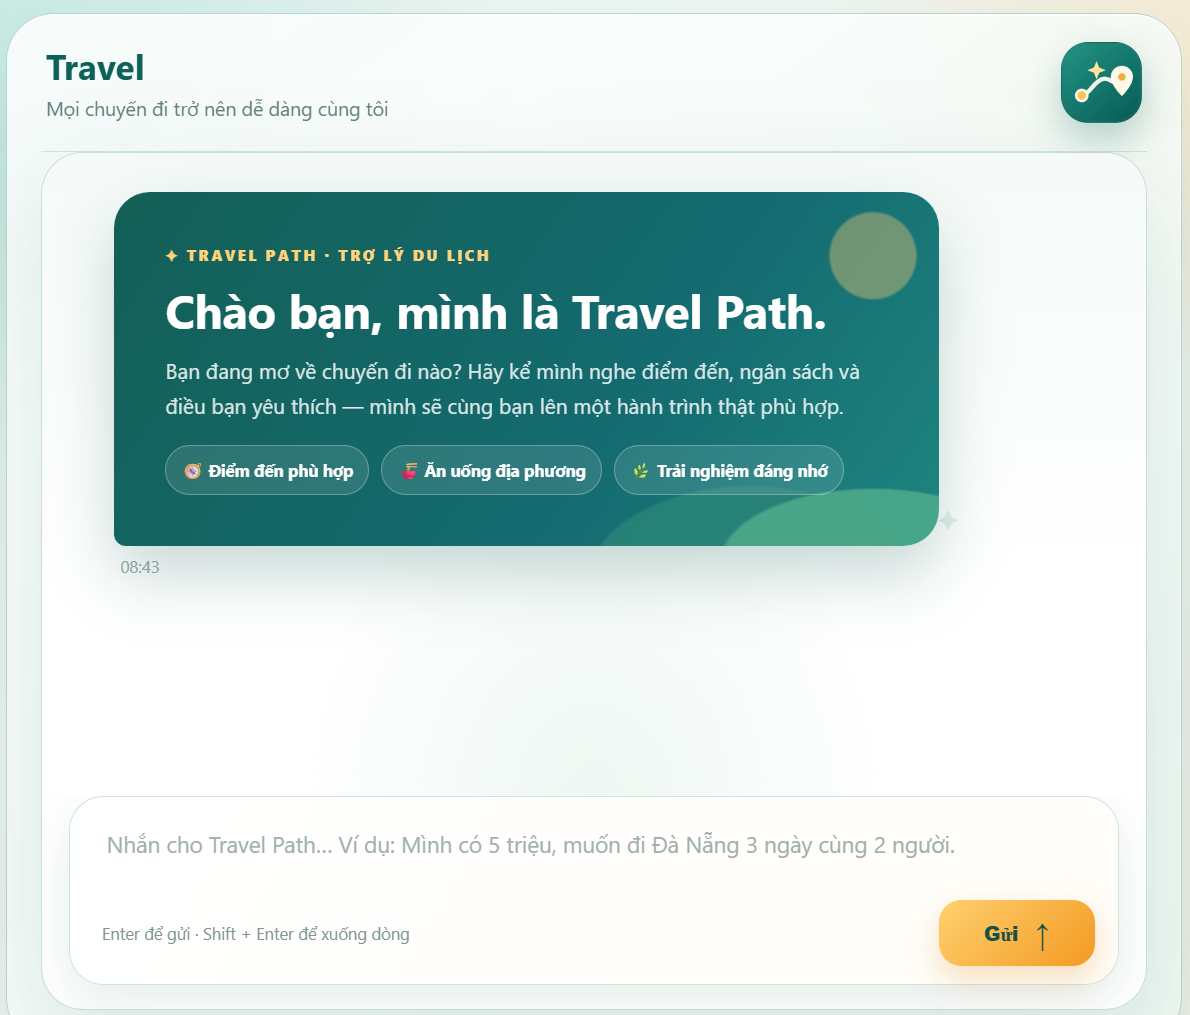
\includegraphics[width=0.94\textwidth,height=0.63\textheight,keepaspectratio]{Bao_cao_Travel_Path_assets/ui_chat.png}
\caption{Giao diện trò chuyện Travel Path trong bản thử nghiệm}
\label{fig:ui-chat}
\end{figure}
Hình~\ref{fig:ui-chat} cho thấy người dùng có thể bắt đầu bằng câu mô tả tự do thay vì phải điền toàn bộ thông tin vào nhiều biểu mẫu. Thẻ chào nêu rõ các yếu tố người dùng nên cung cấp; vùng nhập nằm cố định ở cuối khung trò chuyện giúp tiếp tục trao đổi. Ảnh chụp được cắt từ giao diện để làm rõ vùng ứng dụng chính; các ảnh phụ trang trí hai bên không đưa vào hình này vì không liên quan đến luồng chức năng.

\subsection{Giao diện đăng nhập}
\begin{figure}[H]
\centering
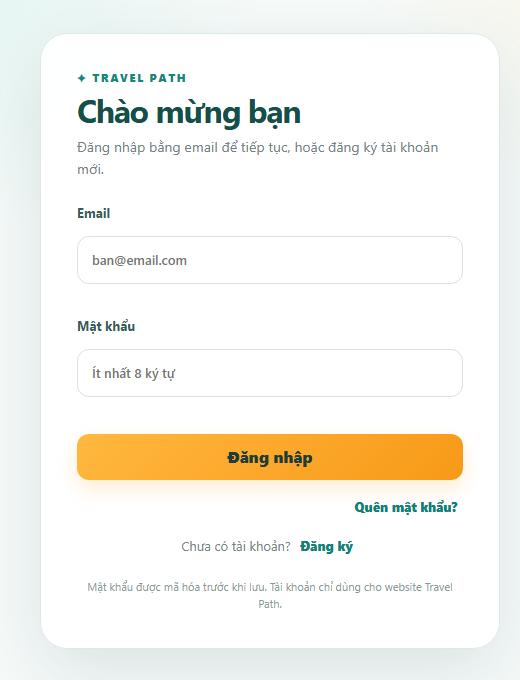
\includegraphics[width=0.82\textwidth,height=0.55\textheight,keepaspectratio]{Bao_cao_Travel_Path_assets/ui_login.png}
\caption{Trang đăng nhập của ứng dụng web Travel Path}
\label{fig:ui-login}
\end{figure}
Hình~\ref{fig:ui-login} thể hiện trang xác thực với hai trường email và mật khẩu, nút đăng nhập, lối dẫn đến đăng ký và khôi phục mật khẩu. Trang riêng giúp hệ thống áp dụng yêu cầu đăng nhập trước khi vào trang chính và tách luồng quên mật khẩu khỏi luồng tạo tài khoản. Đây là ảnh chụp trang thật tại địa chỉ chạy cục bộ của ứng dụng, không chứa thông tin tài khoản đã điền.

\subsection{Giao diện kết quả kế hoạch và ngân sách}
\begin{figure}[H]
\centering
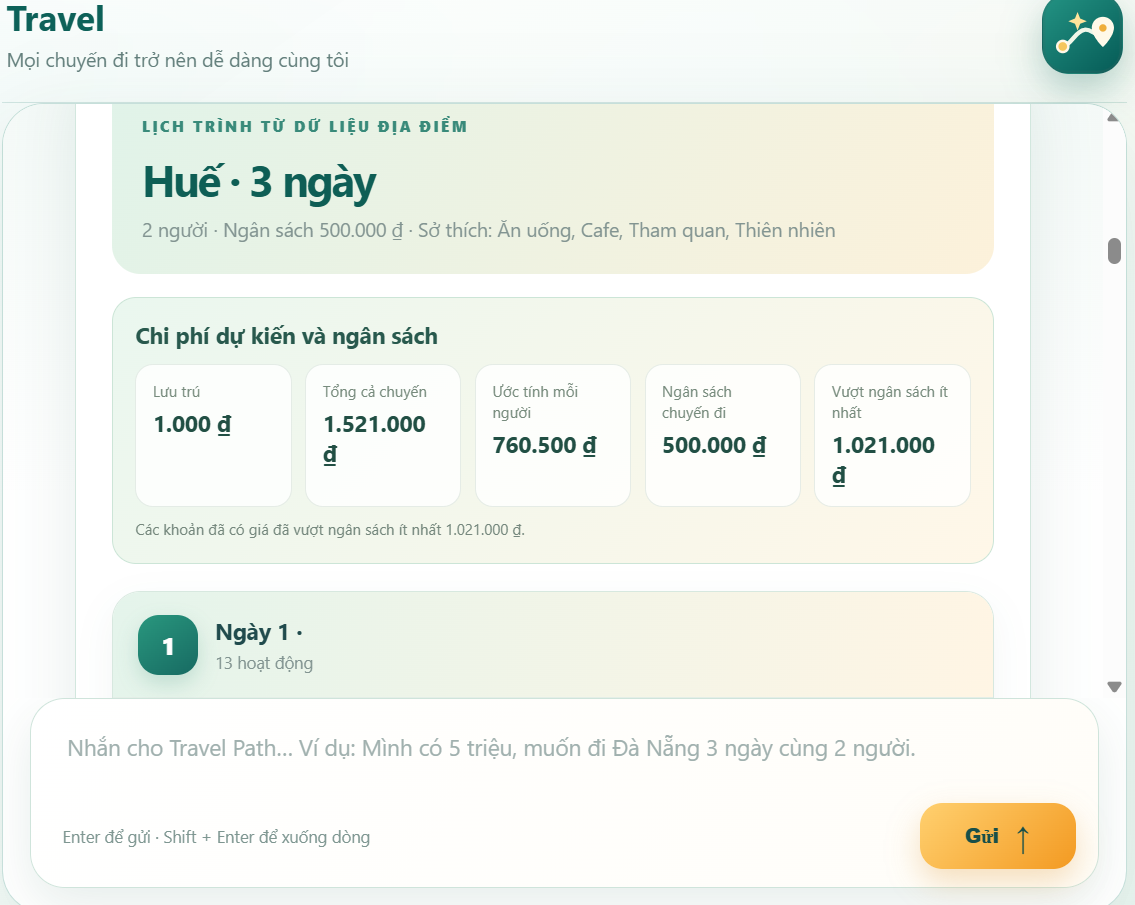
\includegraphics[width=0.94\textwidth,height=0.66\textheight,keepaspectratio]{Bao_cao_Travel_Path_assets/ui_plan_budget.png}
\caption{Khu vực tóm tắt ngân sách trong một plan được hiển thị trên web}
\label{fig:ui-budget}
\end{figure}
Hình~\ref{fig:ui-budget} cho thấy plan được chia thành phần tiêu đề chuyến đi, tổng hợp chi phí và nội dung theo ngày. Trong ví dụ chụp màn hình, tổng dự kiến là 1.521.000~đ trong khi ngân sách nhập là 500.000~đ; phần cảnh báo hiển thị mức vượt tối thiểu 1.021.000~đ. Con số này minh họa cách giao diện trình bày chênh lệch ở một plan cụ thể, không phải kết quả kiểm thử đại diện cho mọi dữ liệu. Nó cũng cho thấy hệ thống cần ưu tiên gợi ý phương án giảm chi và làm rõ các khoản còn thiếu trước khi người dùng xác nhận lịch trình.

\section{Đối chiếu các chức năng theo mã nguồn}
\begin{table}[H]
\centering
\caption{Ma trận chức năng và bằng chứng trong cấu trúc dự án}
\label{tab:implementation}
\begin{tabularx}{\textwidth}{p{3.2cm}p{4.3cm}Y}
\toprule
\textbf{Chức năng} & \textbf{Bằng chứng cấu trúc} & \textbf{Diễn giải trạng thái} \\
\midrule
Đăng nhập/đăng ký & Trang \,\code{account.html}; API xác thực trong backend & Có giao diện và các tuyến API; gửi OTP thực tế phụ thuộc cấu hình email. \\
Chat và lập plan & \,\code{index.html}, \,\code{assistant.js}, \,\code{/api/chat-plan} & Nhận câu chat và tạo lịch trình dựa trên dữ liệu sẵn sàng. \\
Lập kế hoạch & \,\code{planner.html}, API \,\code{/api/plan} & Tạo lịch theo đầu vào và dữ liệu địa điểm; tuyến đường có thể dùng phương án dự phòng. \\
Lịch sử plan & \,\code{history.html}, bảng \,\code{saved\_travel\_plans} & Plan gắn với tài khoản, hỗ trợ xem lại. \\
Quản trị & \,\code{admin.html}, kiểm tra role ở backend & Chỉ tài khoản có quyền quản trị được truy cập API quản trị. \\
PDF & Hành động xuất trên giao diện kế hoạch & Tạo tệp PDF từ plan được hiển thị; chất lượng bố cục cần kiểm tra trên nội dung dài/ngắn. \\
\bottomrule
\end{tabularx}
\end{table}
\noindent Bảng~\ref{tab:implementation} tổng hợp kết quả rà soát mã nguồn thay vì ghi nhận một đợt chạy thử có số liệu. Tên tệp và tuyến API được dùng để chỉ vị trí chức năng; riêng email OTP còn phụ thuộc cấu hình SMTP. Cách trình bày này phân biệt tính năng hiện diện trong dự án với trạng thái vận hành thực tế của các dịch vụ ngoài.

\section{Phân tích ví dụ tính chi phí}
Xét ví dụ minh họa khách sạn có giá từ 80.000~đ đến 300.000~đ/đêm, hành trình 3 đêm. Giá giữa là $(80.000+300.000)/2=190.000$~đ/đêm; chi phí phòng dự kiến là $190.000\times3=570.000$~đ cho phòng, không nhân với số người theo quy tắc yêu cầu. Nếu quán ăn có khoảng giá 10.000--20.000~đ/phần, giá đại diện là 15.000~đ/phần; sau hệ số 2 là 30.000~đ/người cho mỗi lần ăn. Với nhóm 3 người, chi phí dự kiến của lần ăn đó là 90.000~đ. Đây là phép tính minh họa cho quy tắc trong hệ thống, chưa bao gồm số phòng bổ sung hoặc biến động giá thực tế.

\begin{table}[H]
\centering
\caption{Ví dụ minh họa cách tính lưu trú và bữa ăn}
\label{tab:cost-example}
\begin{tabularx}{\textwidth}{p{3.1cm}p{3.8cm}p{3.2cm}Y}
\toprule
\textbf{Khoản} & \textbf{Dữ liệu đầu vào} & \textbf{Phép tính} & \textbf{Ước tính} \\
\midrule
Khách sạn & 80.000--300.000~đ/đêm; 3 đêm; 3 người & Trung điểm $190.000\times3$ & 570.000~đ/phòng; không nhân số người \\
Bữa ăn & 10.000--20.000~đ/phần; 3 người & Trung điểm 15.000 $\times2\times3$ & 90.000~đ cho một bữa của nhóm \\
Tổng ví dụ & Một lần lưu trú + một bữa & 570.000 + 90.000 & 660.000~đ, chưa tính vé và chi phí khác \\
\bottomrule
\end{tabularx}
\end{table}
\noindent Bảng~\ref{tab:cost-example} giải thích vì sao chi phí phòng không thay đổi theo số người trong phép tính hiện tại: đơn giá trong DB được hiểu là giá phòng/đêm, còn số người chỉ tham gia vào khoản ăn uống theo phần. Tổng 660.000~đ chỉ là phép cộng hai khoản đã nêu. Không thể kết luận tổng chuyến đi nằm trong ngân sách khi vé, đi lại và một số bữa chưa được đưa vào.

\section{Kịch bản nghiệm thu đề xuất}
\begin{table}[H]
\centering
\caption{Kịch bản kiểm tra chức năng cần thực hiện trước khi nghiệm thu}
\label{tab:acceptance}
\begin{tabularx}{\textwidth}{p{0.9cm}p{4.5cm}p{4.2cm}Y}
\toprule
\textbf{STT} & \textbf{Tình huống} & \textbf{Kết quả mong đợi} & \textbf{Trạng thái trong báo cáo} \\
\midrule
1 & Đăng nhập email chưa tồn tại & Báo tài khoản chưa tồn tại và hướng dẫn đăng ký & Kịch bản đề xuất; chưa ghi nhận chạy kiểm thử. \\
2 & Đăng ký email đã có tài khoản & Báo tài khoản đã tồn tại và hướng dẫn đăng nhập & Kịch bản đề xuất; chưa ghi nhận chạy kiểm thử. \\
3 & Nhập OTP sai hoặc hết hạn & Từ chối xác minh, cho biết cần gửi lại OTP & Kịch bản đề xuất; cần thử với SMTP hoạt động. \\
4 & Tạo plan với giá khách sạn dạng khoảng & Lấy trung điểm và nhân số đêm, không nhân số người & Đối chiếu công thức; ví dụ ở Bảng~\ref{tab:cost-example}. \\
5 & Giá một bữa ăn dạng khoảng & Lấy trung điểm, nhân hệ số 2 và số người & Đối chiếu công thức; ví dụ ở Bảng~\ref{tab:cost-example}. \\
6 & Plan vượt ngân sách & Hiển thị tổng, mức vượt và cho phép tối ưu/tạo lại plan & Giao diện minh họa ở Hình~\ref{fig:ui-budget}. \\
7 & Lưu và mở lại plan & Chỉ người sở hữu xem được plan của mình & Kịch bản đề xuất; chưa ghi nhận chạy kiểm thử. \\
\bottomrule
\end{tabularx}
\end{table}
\noindent Bảng~\ref{tab:acceptance} chuyển các yêu cầu trọng yếu thành tình huống có thể kiểm tra. Cột trạng thái cố ý phân biệt việc đối chiếu công thức/mã nguồn với kết quả thực nghiệm. Trước nghiệm thu, cần thực thi từng kịch bản trong môi trường đủ dịch vụ, ghi lại dữ liệu đầu vào, kết quả quan sát và ảnh chụp bằng chứng; đặc biệt, kiểm thử OTP cần cấu hình email hợp lệ.

\section{Hạn chế và hướng phát triển}
\subsection{Hạn chế}
\begin{itemize}
  \item Chất lượng lịch trình phụ thuộc độ đầy đủ, địa chỉ và mức cập nhật của dữ liệu địa điểm; bản ghi sai địa bàn hoặc sai ảnh sẽ làm giảm độ tin cậy.
  \item Giá trên DB có thể là khoảng, một mức hoặc bị thiếu; giá ước tính không bảo đảm khớp giá tại thời điểm đặt dịch vụ.
  \item Tuyến đường dự phòng theo khoảng cách địa lý không phản ánh đường đi, giao thông hay thời gian thực.
  \item Mô hình ngôn ngữ cục bộ có thể diễn giải sai câu mơ hồ; nhánh luật và bước hỏi lại giúp giảm nhưng không loại bỏ hoàn toàn lỗi.
  \item Báo cáo chưa trình bày kết quả chạy kiểm thử có đo lường, thử nghiệm người dùng, đánh giá chất lượng gợi ý hoặc tải hệ thống. Những kết luận định lượng về độ chính xác/hiệu năng vì vậy chưa được đưa ra.
\end{itemize}

\subsection{Hướng phát triển}
Các hướng tiếp theo gồm kiểm tra và chuẩn hóa địa chỉ theo địa giới hành chính hiện hành; theo dõi nguồn và thời điểm cập nhật giá; bổ sung khả năng nhập số phòng khi cần; ưu tiên chọn phương án tiết kiệm hơn khi người dùng đặt trần ngân sách; kiểm thử tự động các luồng xác thực, lập plan và chi phí; đo độ phù hợp gợi ý với người dùng; cải thiện PDF để mang theo hình địa điểm và bố cục ổn định; đồng thời hoàn thiện HTTPS, cấu hình secrets, sao lưu và giám sát trước khi triển khai công khai.

\section{Kết luận}
Đề tài đã xây dựng mô hình ứng dụng web Travel Path kết hợp giao diện hội thoại, bộ lập lịch dựa trên dữ liệu, cơ sở dữ liệu địa điểm, ước tính chi phí, xác thực tài khoản và lịch sử kế hoạch. Báo cáo trình bày ba chương, có sơ đồ thiết kế vẽ bằng TikZ, bảng LaTeX và hình chụp giao diện web ở phần kết quả. Mỗi hình và bảng đều được đánh số theo chương và giải thích trong nội dung.

Kết quả hiện có thể hiện nền tảng kỹ thuật và luồng chức năng của đồ án, chưa thay thế đánh giá qua kiểm thử và thử nghiệm người dùng. Bước quan trọng tiếp theo là thực hiện ma trận nghiệm thu ở Bảng~\ref{tab:acceptance}, kiểm tra dữ liệu địa điểm, hiệu chỉnh phần tối ưu ngân sách và lưu bằng chứng thực nghiệm để báo cáo có thể kết luận dựa trên kết quả đo được.

% =============================================================================
% TÀI LIỆU THAM KHẢO (không tạo chương thứ tư)
% =============================================================================
\clearpage
\addcontentsline{toc}{chapter}{Tài liệu tham khảo}
\begin{thebibliography}{99}
\bibitem{q1} Thủ tướng Chính phủ, \emph{Quyết định số 147/QĐ-TTg phê duyệt Chiến lược phát triển du lịch Việt Nam đến năm 2030}, 2020. \url{https://vanban.chinhphu.vn/?docid=198927\&pageid=27160\&tagid=6\&type=1}
\bibitem{q2} Quốc hội, \emph{Luật Du lịch số 09/2017/QH14}, 2017. \url{https://vanban.chinhphu.vn/?docid=190290\&pageid=27160}
\bibitem{q3} Cục Thống kê, \emph{Thông cáo báo chí tình hình kinh tế -- xã hội quý IV và năm 2025}, 2026. \url{https://www.nso.gov.vn/tin-tuc-thong-ke/2026/01/thong-cao-bao-chi-tinh-hinh-kinh-te-xa-hoi-quy-iv-va-nam-2025/}
\bibitem{q4} Cục Du lịch Quốc gia Việt Nam, \emph{International visitor statistics dashboard}, truy cập 2026. \url{https://vietnamtourism.gov.vn/en/statistic/international}
\bibitem{q5} Quốc hội, \emph{Nghị quyết số 202/2025/QH15 về sắp xếp đơn vị hành chính cấp tỉnh}, 2025. \url{https://vanban.chinhphu.vn/?classid=0\&docid=213930\&pageid=27160}
\bibitem{q6} P. Resnick and H. R. Varian, ``Recommender Systems,'' \emph{Communications of the ACM}, vol. 40, no. 3, pp. 56--58, 1997. \url{https://doi.org/10.1145/245108.245121}
\bibitem{q7} R. Burke, ``Hybrid Recommender Systems: Survey and Experiments,'' \emph{User Modeling and User-Adapted Interaction}, vol. 12, pp. 331--370, 2002. \url{https://doi.org/10.1023/A:1021240730564}
\bibitem{q8} Sebastián Ramírez et al., \emph{FastAPI Documentation: Tutorial}, truy cập 2026. \url{https://fastapi.tiangolo.com/tutorial/}
\bibitem{q9} Sebastián Ramírez et al., \emph{FastAPI Documentation: First Steps}, truy cập 2026. \url{https://fastapi.tiangolo.com/tutorial/first-steps/}
\bibitem{q10} OpenAPI Initiative, \emph{OpenAPI Specification}, truy cập 2026. \url{https://spec.openapis.org/oas/}
\bibitem{q11} PostgreSQL Global Development Group, \emph{PostgreSQL 16 Documentation: What Is PostgreSQL?}, 2023. \url{https://www.postgresql.org/docs/16/intro-whatis.html}
\bibitem{q12} PostGIS Project Steering Committee, \emph{PostGIS Documentation}, truy cập 2026. \url{https://www.postgis.net/documentation/manual/}
\bibitem{q13} Docker Inc., \emph{Docker Compose overview}, truy cập 2026. \url{https://docs.docker.com/get-started/docker-concepts/the-basics/what-is-docker-compose/}
\bibitem{q14} Ollama, \emph{Ollama API documentation}, truy cập 2026. \url{https://github.com/ollama/ollama/blob/main/docs/api.md}
\bibitem{q15} OWASP Foundation, \emph{Password Storage Cheat Sheet}, truy cập 2026. \url{https://cheatsheetseries.owasp.org/cheatsheets/Password_Storage_Cheat_Sheet.html}
\bibitem{q16} OWASP Foundation, \emph{Authentication Cheat Sheet}, truy cập 2026. \url{https://cheatsheetseries.owasp.org/cheatsheets/Authentication_Cheat_Sheet.html}
\bibitem{q17} OWASP Foundation, \emph{Session Management Cheat Sheet}, truy cập 2026. \url{https://cheatsheetseries.owasp.org/cheatsheets/Session_Management_Cheat_Sheet.html}
\bibitem{q18} Python Software Foundation, \emph{hashlib -- Secure hashes and message digests}, truy cập 2026. \url{https://docs.python.org/3/library/hashlib.html}
\bibitem{q19} Project OSRM, \emph{OSRM HTTP API Documentation}, truy cập 2026. \url{https://project-osrm.org/docs/v26.5.0/index.html}
\end{thebibliography}

\end{document}
